% Options for packages loaded elsewhere
\PassOptionsToPackage{unicode}{hyperref}
\PassOptionsToPackage{hyphens}{url}
%
\documentclass[
]{article}
\usepackage{amsmath,amssymb}
\usepackage{lmodern}
\usepackage{iftex}
\ifPDFTeX
  \usepackage[T1]{fontenc}
  \usepackage[utf8]{inputenc}
  \usepackage{textcomp} % provide euro and other symbols
\else % if luatex or xetex
  \usepackage{unicode-math}
  \defaultfontfeatures{Scale=MatchLowercase}
  \defaultfontfeatures[\rmfamily]{Ligatures=TeX,Scale=1}
\fi
% Use upquote if available, for straight quotes in verbatim environments
\IfFileExists{upquote.sty}{\usepackage{upquote}}{}
\IfFileExists{microtype.sty}{% use microtype if available
  \usepackage[]{microtype}
  \UseMicrotypeSet[protrusion]{basicmath} % disable protrusion for tt fonts
}{}
\makeatletter
\@ifundefined{KOMAClassName}{% if non-KOMA class
  \IfFileExists{parskip.sty}{%
    \usepackage{parskip}
  }{% else
    \setlength{\parindent}{0pt}
    \setlength{\parskip}{6pt plus 2pt minus 1pt}}
}{% if KOMA class
  \KOMAoptions{parskip=half}}
\makeatother
\usepackage{xcolor}
\usepackage{longtable,booktabs,array}
\usepackage{calc} % for calculating minipage widths
% Correct order of tables after \paragraph or \subparagraph
\usepackage{etoolbox}
\makeatletter
\patchcmd\longtable{\par}{\if@noskipsec\mbox{}\fi\par}{}{}
\makeatother
% Allow footnotes in longtable head/foot
\IfFileExists{footnotehyper.sty}{\usepackage{footnotehyper}}{\usepackage{footnote}}
\makesavenoteenv{longtable}
\usepackage{graphicx}
\makeatletter
\def\maxwidth{\ifdim\Gin@nat@width>\linewidth\linewidth\else\Gin@nat@width\fi}
\def\maxheight{\ifdim\Gin@nat@height>\textheight\textheight\else\Gin@nat@height\fi}
\makeatother
% Scale images if necessary, so that they will not overflow the page
% margins by default, and it is still possible to overwrite the defaults
% using explicit options in \includegraphics[width, height, ...]{}
\setkeys{Gin}{width=\maxwidth,height=\maxheight,keepaspectratio}
% Set default figure placement to htbp
\makeatletter
\def\fps@figure{htbp}
\makeatother
\setlength{\emergencystretch}{3em} % prevent overfull lines
\providecommand{\tightlist}{%
  \setlength{\itemsep}{0pt}\setlength{\parskip}{0pt}}
\setcounter{secnumdepth}{-\maxdimen} % remove section numbering
\ifLuaTeX
  \usepackage{selnolig}  % disable illegal ligatures
\fi
\IfFileExists{bookmark.sty}{\usepackage{bookmark}}{\usepackage{hyperref}}
\IfFileExists{xurl.sty}{\usepackage{xurl}}{} % add URL line breaks if available
\urlstyle{same} % disable monospaced font for URLs
\hypersetup{
  hidelinks,
  pdfcreator={LaTeX via pandoc}}

\author{}
\date{}

\begin{document}

\begin{titlepage}
    \centering
    {\LARGE\textbf{Software Requirements Specification (SRS)}\par}
    \vspace{1cm}
    {\Large For\par}
    \vspace{0.5cm}
    {\Large\textbf{Box.com Discovery Bates Namer: Cloud Integration}\par}
    \vspace{1.5cm}
    {\large Version: 3.0.0\par}
    \vspace{1.5cm}
    Prepared by:\par
    Chiemela Eziechile-Nwoke, James Chau,\par 
    Everest McNally, Benjamin Geiser, Miguel Campos\par
    \vspace{1.5cm}
    \textbf{Santa Barbara Public Defender's Office}\par
    \vspace{0.5cm}
    May 2025\par
    \vfill
\end{titlepage}

\tableofcontents
\newpage
\hypertarget{software-requirements-specification-srs}{%
\section{\texorpdfstring{\textbf{Software Requirements Specification
(SRS)}}{Software Requirements Specification (SRS)}}\label{software-requirements-specification-srs}}

\textbf{For}\\
\textbf{Box.com Discovery Bates Namer: Cloud Integration}

\textbf{Version:} 3.0.0\\
\textbf{Prepared by:}\\
Chiemela Eziechile-Nwoke, James Chau, Everest McNally, Benjamin Geiser,
Miguel Campos

\textbf{Santa Barbara Public Defender\textquotesingle s Office}\\
\textbf{May 2025}

\hypertarget{introduction}{%
\subsection{\texorpdfstring{\textbf{1.
Introduction}}{1. Introduction}}\label{introduction}}

\hypertarget{purpose}{%
\subsubsection{\texorpdfstring{\textbf{1.1
Purpose}}{1.1 Purpose}}\label{purpose}}

The Box.com Discovery Bates Namer is a cloud-based system designed to
automate the processing, renaming, and organization of legal discovery
documents for the Santa Barbara Public Defender\textquotesingle s
Office. This document specifies the functional and non-functional
requirements for the system, which integrates Box.com with Azure cloud
services to provide a secure, scalable, and efficient solution for
managing discovery files.

Key objectives include:

\begin{itemize}
\tightlist
\item
  Eliminating manual file renaming processes
\item
  Ensuring CJIS and HIPAA compliance
\item
  Reducing processing time from hours to minutes
\item
  Providing audit trails for all file operations
\end{itemize}

\hypertarget{document-conventions}{%
\subsubsection{\texorpdfstring{\textbf{1.2 Document
Conventions}}{1.2 Document Conventions}}\label{document-conventions}}

This document uses the following formatting conventions:

\begin{itemize}
\item
  \textbf{Bold text} indicates key terms and system components
\item
  \emph{Italicized text} denotes references to external systems or
  components
\item
  \texttt{Monospace} highlights technical parameters and code references
\item
  \begin{quote}
  Blockquotes show important notes or exceptions
  \end{quote}
\end{itemize}

All requirements are numbered using the format
{[}Section{]}.{[}Subsection{]}.{[}Requirement\#{]} (e.g., 4.1.3.1).

\hypertarget{intended-audience-and-reading-suggestions}{%
\subsubsection{\texorpdfstring{\textbf{1.3 Intended Audience and Reading
Suggestions}}{1.3 Intended Audience and Reading Suggestions}}\label{intended-audience-and-reading-suggestions}}

\begin{longtable}[]{@{}
  >{\raggedright\arraybackslash}p{(\columnwidth - 4\tabcolsep) * \real{0.3022}}
  >{\raggedright\arraybackslash}p{(\columnwidth - 4\tabcolsep) * \real{0.3769}}
  >{\raggedright\arraybackslash}p{(\columnwidth - 4\tabcolsep) * \real{0.3209}}@{}}
\toprule()
\begin{minipage}[b]{\linewidth}\raggedright
Audience
\end{minipage} & \begin{minipage}[b]{\linewidth}\raggedright
Focus Areas
\end{minipage} & \begin{minipage}[b]{\linewidth}\raggedright
Suggested Reading
\end{minipage} \\
\midrule()
\endhead
Developers & Implementation details & Sections 3, 4, 5.3 \\
Legal Staff & User workflows & 2.3, 3.1, 4.1 \\
IT Administrators & System maintenance & 2.5, 5.3, 6.1 \\
Project Managers & Overall scope & 1.4, 2.1, 5.5 \\
\bottomrule()
\end{longtable}

\hypertarget{product-scope}{%
\subsubsection{\texorpdfstring{\textbf{1.4 Product
Scope}}{1.4 Product Scope}}\label{product-scope}}

\textbf{Included Features:}

\begin{itemize}
\tightlist
\item
  Automated detection of new file uploads in designated Box folders
\item
  AI-powered extraction of Bates numbers using Azure Form Recognizer
\item
  File renaming following strict naming conventions
\item
  Secure file movement to case-specific folders
\item
  Multi-channel error notifications (email + SMS)
\end{itemize}

\textbf{Excluded Features:}

\begin{itemize}
\tightlist
\item
  Processing of non-PDF documents
\item
  Handwritten Bates number recognition (v1.0)
\item
  Local file processing outside Box/Azure ecosystem
\end{itemize}

\hypertarget{definitions-acronyms-and-abbreviations}{%
\subsubsection{\texorpdfstring{\textbf{1.5 Definitions, Acronyms, and
Abbreviations}}{1.5 Definitions, Acronyms, and Abbreviations}}\label{definitions-acronyms-and-abbreviations}}

\begin{longtable}[]{@{}
  >{\raggedright\arraybackslash}p{(\columnwidth - 2\tabcolsep) * \real{0.1839}}
  >{\raggedright\arraybackslash}p{(\columnwidth - 2\tabcolsep) * \real{0.8161}}@{}}
\toprule()
\begin{minipage}[b]{\linewidth}\raggedright
Term
\end{minipage} & \begin{minipage}[b]{\linewidth}\raggedright
Definition
\end{minipage} \\
\midrule()
\endhead
ESI & Electronically Stored Information \\
CJIS & Criminal Justice Information Services \\
OCR & Optical Character Recognition \\
RBAC & Role-Based Access Control \\
PHI & Protected Health Information \\
\bottomrule()
\end{longtable}

\hypertarget{references}{%
\subsubsection{\texorpdfstring{\textbf{1.6
References}}{1.6 References}}\label{references}}

\begin{enumerate}
\def\labelenumi{\arabic{enumi}.}
\tightlist
\item
  Box API Documentation v2.0
\item
  Azure HIPAA Compliance Whitepaper
\item
  CJIS Security Policy v5.9
\end{enumerate}

\hypertarget{overall-description}{%
\subsection{\texorpdfstring{\textbf{2. Overall
Description}}{2. Overall Description}}\label{overall-description}}

\hypertarget{system-analysis}{%
\subsubsection{\texorpdfstring{\textbf{2.1 System
Analysis}}{2.1 System Analysis}}\label{system-analysis}}

\textbf{Current Workflow Pain Points:}

\begin{itemize}
\tightlist
\item
  Staff spends 3-5 hours daily manually renaming files
\item
  12\% error rate in manual Bates number transcription
\item
  No centralized audit trail for file changes
\end{itemize}

\textbf{Proposed Solution Architecture:}

\hypertarget{product-perspective}{%
\subsubsection[\textbf{2.2 Product
Perspective}]{\texorpdfstring{\protect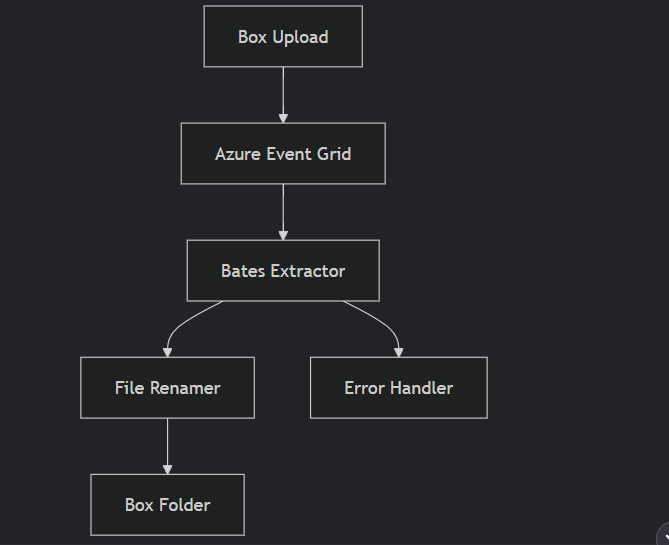
\includegraphics[width=6.5in,height=5.29514in]{image1.png}\textbf{2.2
Product
Perspective}}{2.2 Product Perspective}}\label{product-perspective}}

\textbf{System Interfaces:}

\begin{enumerate}
\def\labelenumi{\arabic{enumi}.}
\item
  \textbf{Box.com}

  \begin{itemize}
  \tightlist
  \item
    Primary file storage
  \item
    Webhook notifications
  \end{itemize}
\item
  \textbf{Azure Services}

  \begin{itemize}
  \tightlist
  \item
    Functions: Serverless processing
  \item
    Blob Storage: Temporary file cache
  \item
    Key Vault: Credential management
  \end{itemize}
\end{enumerate}

\hypertarget{product-functions}{%
\subsubsection{\texorpdfstring{\textbf{2.3 Product
Functions}}{2.3 Product Functions}}\label{product-functions}}

\begin{longtable}[]{@{}
  >{\raggedright\arraybackslash}p{(\columnwidth - 4\tabcolsep) * \real{0.1888}}
  >{\raggedright\arraybackslash}p{(\columnwidth - 4\tabcolsep) * \real{0.3861}}
  >{\raggedright\arraybackslash}p{(\columnwidth - 4\tabcolsep) * \real{0.4251}}@{}}
\toprule()
\begin{minipage}[b]{\linewidth}\raggedright
Function
\end{minipage} & \begin{minipage}[b]{\linewidth}\raggedright
Description
\end{minipage} & \begin{minipage}[b]{\linewidth}\raggedright
Technical Implementation
\end{minipage} \\
\midrule()
\endhead
File Intake & Monitor Box folder for new uploads & Box webhook → Azure
Event Grid \\
Bates Extraction & Extract numbers from PDFs & Azure Form Recognizer +
custom regex \\
Validation & Verify Bates sequence & Python validation service \\
Renaming & Apply naming convention & Box API v2.0 \\
\bottomrule()
\end{longtable}

\hypertarget{user-classes-and-characteristics}{%
\subsubsection{\texorpdfstring{\textbf{2.4 User Classes and
Characteristics}}{2.4 User Classes and Characteristics}}\label{user-classes-and-characteristics}}

\textbf{Primary Users:}

\begin{enumerate}
\def\labelenumi{\arabic{enumi}.}
\item
  \textbf{Legal Assistants}

  \begin{itemize}
  \tightlist
  \item
    Upload 50-100 files daily
  \item
    Require simple interface
  \item
    Need immediate error feedback
  \end{itemize}
\item
  \textbf{IT Administrators}

  \begin{itemize}
  \tightlist
  \item
    Manage system configurations
  \item
    Monitor processing queues
  \item
    Handle credential rotation
  \end{itemize}
\end{enumerate}

\hypertarget{operating-environment}{%
\subsubsection{\texorpdfstring{\textbf{2.5 Operating
Environment}}{2.5 Operating Environment}}\label{operating-environment}}

\textbf{Cloud Infrastructure:}

\begin{itemize}
\tightlist
\item
  Azure East US 2 region
\item
  Python 3.11 runtime
\item
  Box Enterprise Plan
\end{itemize}

\textbf{Client Requirements:}

\begin{itemize}
\tightlist
\item
  Modern web browser (Chrome 110+)
\item
  Box-approved mobile app for notifications
\end{itemize}

\hypertarget{external-interface-requirements}{%
\subsection{\texorpdfstring{\textbf{3. External Interface
Requirements}}{3. External Interface Requirements}}\label{external-interface-requirements}}

\hypertarget{user-interfaces}{%
\subsubsection{\texorpdfstring{\textbf{3.1 User
Interfaces}}{3.1 User Interfaces}}\label{user-interfaces}}

\textbf{Box.com Web Interface:}

\begin{itemize}
\tightlist
\item
  Upload area: "Discovery\_Uploads" folder
\item
  Status indicators:

  \begin{itemize}
  \tightlist
  \item
    Processed
  \item
    Needs Review
  \item
    Failed
  \end{itemize}
\end{itemize}

\hypertarget{software-interfaces}{%
\subsubsection{\texorpdfstring{\textbf{3.2 Software
Interfaces}}{3.2 Software Interfaces}}\label{software-interfaces}}

\begin{longtable}[]{@{}
  >{\raggedright\arraybackslash}p{(\columnwidth - 6\tabcolsep) * \real{0.3178}}
  >{\raggedright\arraybackslash}p{(\columnwidth - 6\tabcolsep) * \real{0.2000}}
  >{\raggedright\arraybackslash}p{(\columnwidth - 6\tabcolsep) * \real{0.2498}}
  >{\raggedright\arraybackslash}p{(\columnwidth - 6\tabcolsep) * \real{0.2324}}@{}}
\toprule()
\begin{minipage}[b]{\linewidth}\raggedright
Interface
\end{minipage} & \begin{minipage}[b]{\linewidth}\raggedright
Protocol
\end{minipage} & \begin{minipage}[b]{\linewidth}\raggedright
Data Format
\end{minipage} & \begin{minipage}[b]{\linewidth}\raggedright
Security
\end{minipage} \\
\midrule()
\endhead
Box API & HTTPS & JSON & OAuth 2.0 \\
Azure Functions & HTTP & Binary & Azure AD \\
SMTP Server & TLS 1.2+ & MIME & SPF/DKIM \\
\bottomrule()
\end{longtable}

\hypertarget{communications-interfaces}{%
\subsubsection{\texorpdfstring{\textbf{3.3 Communications
Interfaces}}{3.3 Communications Interfaces}}\label{communications-interfaces}}

\textbf{Error Notification Flow:}

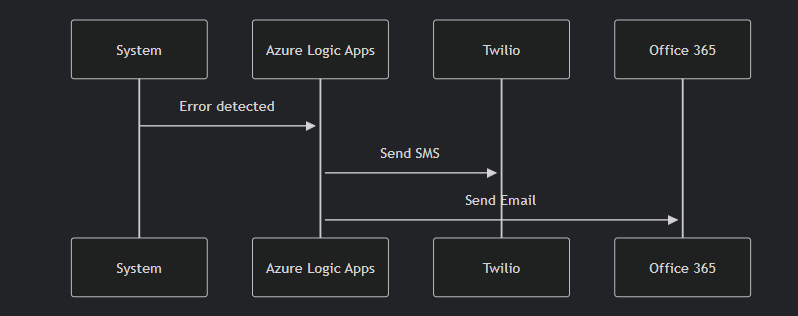
\includegraphics[width=6.5in,height=2.57361in]{image2.png}

\hypertarget{system-features}{%
\subsection{\texorpdfstring{\textbf{4. System
Features}}{4. System Features}}\label{system-features}}

\hypertarget{file-upload-processing}{%
\subsubsection{\texorpdfstring{\textbf{4.1 File Upload \&
Processing}}{4.1 File Upload \& Processing}}\label{file-upload-processing}}

\textbf{4.1.1 File Size Validation}

\begin{itemize}
\tightlist
\item
  Maximum: 100 MB per file
\item
  Minimum: 10 KB
\item
  Error: "FILE\_SIZE\_EXCEEDED"
\end{itemize}

\textbf{4.1.2 File Type Checking}

\begin{itemize}
\tightlist
\item
  Allowed: PDF/A-1b, PDF/A-2u
\item
  Rejected: Password-protected PDFs
\end{itemize}

\hypertarget{bates-number-extraction}{%
\subsubsection{\texorpdfstring{\textbf{4.2 Bates Number
Extraction}}{4.2 Bates Number Extraction}}\label{bates-number-extraction}}

\textbf{4.2.1 AI Model Configuration}

\begin{itemize}
\tightlist
\item
  Training data: 5,000 labeled discovery documents
\item
  Confidence threshold: 85\%
\end{itemize}

\textbf{4.2.2 Fallback Mechanism}

\begin{enumerate}
\def\labelenumi{\arabic{enumi}.}
\tightlist
\item
  Primary: Form Recognizer
\item
  Secondary: Regex pattern
  \texttt{//\textbackslash{}}\texttt{d\{}\texttt{5\}}
\item
  Tertiary: Footer text analysis
\end{enumerate}

\hypertarget{file-renaming-organization}{%
\subsubsection{\texorpdfstring{\textbf{4.3 File Renaming \&
Organization}}{4.3 File Renaming \& Organization}}\label{file-renaming-organization}}

\textbf{Naming Convention Examples:}

\begin{longtable}[]{@{}
  >{\raggedright\arraybackslash}p{(\columnwidth - 2\tabcolsep) * \real{0.3047}}
  >{\raggedright\arraybackslash}p{(\columnwidth - 2\tabcolsep) * \real{0.6953}}@{}}
\toprule()
\begin{minipage}[b]{\linewidth}\raggedright
Original Name
\end{minipage} & \begin{minipage}[b]{\linewidth}\raggedright
New Name
\end{minipage} \\
\midrule()
\endhead
Document1.pdf & 00001-00015\_Disc02\_Document1.pdf \\
Evidence.pdf & 00100-00120\_Disc01\_Evidence.pdf \\
\bottomrule()
\end{longtable}

\textbf{Folder Structure Rules:}

\texttt{/Cases/}\strut \\
\texttt{\ \ \ └──\ PD240123/}\strut \\
\texttt{\ \ \ \ \ \ \ └──\ Discovery/}\strut \\
\texttt{\ \ \ \ \ \ \ \ \ \ \ ├──\ Disc01/}\strut \\
\texttt{\ \ \ \ \ \ \ \ \ \ \ └──\ Disc02/}

\hypertarget{non-functional-requirements}{%
\subsection{\texorpdfstring{\textbf{5. Non-Functional
Requirements}}{5. Non-Functional Requirements}}\label{non-functional-requirements}}

\hypertarget{performance-requirements}{%
\subsubsection{\texorpdfstring{\textbf{5.1 Performance
Requirements}}{5.1 Performance Requirements}}\label{performance-requirements}}

\begin{longtable}[]{@{}
  >{\raggedright\arraybackslash}p{(\columnwidth - 4\tabcolsep) * \real{0.2188}}
  >{\raggedright\arraybackslash}p{(\columnwidth - 4\tabcolsep) * \real{0.4037}}
  >{\raggedright\arraybackslash}p{(\columnwidth - 4\tabcolsep) * \real{0.3775}}@{}}
\toprule()
\begin{minipage}[b]{\linewidth}\raggedright
Metric
\end{minipage} & \begin{minipage}[b]{\linewidth}\raggedright
Requirement
\end{minipage} & \begin{minipage}[b]{\linewidth}\raggedright
Measurement Method
\end{minipage} \\
\midrule()
\endhead
Throughput & 500 files/hour & Azure Monitor \\
Latency & \textless10 sec/file (95th \%ile) & Load testing \\
\bottomrule()
\end{longtable}

\hypertarget{security-requirements}{%
\subsubsection{\texorpdfstring{\textbf{5.2 Security
Requirements}}{5.2 Security Requirements}}\label{security-requirements}}

\textbf{Data Protection:}

\begin{itemize}
\tightlist
\item
  Encryption: AES-256 for files in transit/at rest
\item
  Credential rotation: Every 90 days (Key Vault)
\end{itemize}

\textbf{Access Controls:}

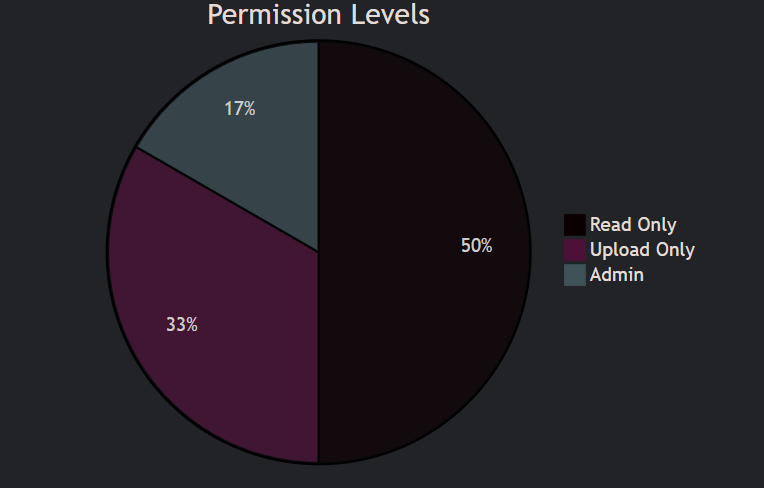
\includegraphics[width=6.5in,height=4.15208in]{image3.png}

\hypertarget{other-requirements}{%
\subsection{\texorpdfstring{\textbf{6. Other
Requirements}}{6. Other Requirements}}\label{other-requirements}}

\hypertarget{legal-compliance}{%
\subsubsection{\texorpdfstring{\textbf{6.1 Legal \&
Compliance}}{6.1 Legal \& Compliance}}\label{legal-compliance}}

\begin{itemize}
\tightlist
\item
  CJIS Audit Log Retention: 7 years
\item
  HIPAA BA Agreement required with Box/Azure
\end{itemize}

\hypertarget{ethical-considerations}{%
\subsubsection{\texorpdfstring{\textbf{6.2 Ethical
Considerations}}{6.2 Ethical Considerations}}\label{ethical-considerations}}

\begin{itemize}
\tightlist
\item
  No AI training on active case files
\item
  Bias testing for handwriting recognition
\end{itemize}

\hypertarget{appendices}{%
\subsection{\texorpdfstring{\textbf{7.
Appendices}}{7. Appendices}}\label{appendices}}

\hypertarget{complete-analysis-models}{%
\subsubsection{\texorpdfstring{\textbf{7.1 Complete Analysis
Models}}{7.1 Complete Analysis Models}}\label{complete-analysis-models}}

\textbf{State Transition Diagram:}

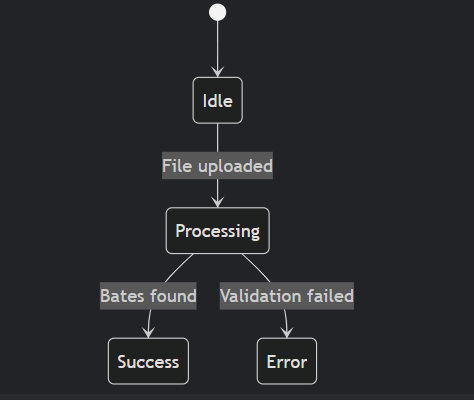
\includegraphics[width=4.93819in,height=4.16725in]{image4.png}

\end{document}
